\chapter{Multivariate PMFs and Densities}
\label{mul}

Individual pmfs $p_X$ and densities $f_X$ don't describe correlations
betwen variables.  We need something more.  We need ways to describe
multivariate distributions.


\subsection{The Multivariate Normal Family of Distributions }
\label{multnormal}

Note to the reader:  This is a more difficult section, but worth putting
extra effort into, as so many statistical applications in computer
science make use of it.  It will seem hard at times, but in the end
won't be too bad.

\subsubsection{Densities}
\label{mvnormdens}

Intuitively, this family has densities which are shaped like
multidimensional bells, just like the univariate normal has the famous
one-dimensional bell shape.  

Let's look at the bivariate case first.  The joint distribution of
$X_1$ and $X_2$ is said to be {\bf bivariate normal} if their density is

\begin{equation}
f_{X,Y}(s,t) = \frac{1}{2\pi \sigma_1 \sigma_2 \sqrt{1-\rho^2}}
e^
{-\frac{1}{2(1-\rho^2)} 
\left [
\frac{(s-\mu_1)^2}{\sigma_1^2} + \frac{(t-\mu_2)^2}{\sigma_2^2} 
-\frac
{2\rho (s-\mu_1)(t-\mu2)}
{\sigma_1 \sigma_2}
\right ]
}, ~ -\infty < s,t < \infty
\end{equation}

{\bf This looks horrible, and it is.  But don't worry, as we won't work
with this directly.  It's important for conceptual reasons, as follows.}

First, note the parameters here:  $\mu_1$, $\mu_2$, $\sigma_1$ and
$\sigma_2$ are the means and standard deviations of X and Y,
while $\rho$ is the correlation between X and Y.  So, we have a
five-parameter family of distributions.

The multivariate normal family of distributions is parameterized by one
vector-valued quantity, the mean $\mu$, and one matrix-valued quantity,
the covariance matrix $\Sigma$.  Specifically, suppose the random vector
$X = (X_1,...,X_k)'$ has a k-variate normal distribution.

The density has this form:

\begin{equation}
\label{bigbell}
f_X(t) = c e^{-0.5 (t-\mu)'\Sigma^{-1}(t-\mu)}
\end{equation}

Here c is a constant, needed to make the density integrate to 1.0.  It
turns out that 

\begin{equation}
c = \frac
{1}
{(2\pi)^{k/2} \sqrt{det(\Sigma)}}
\end{equation}

but we'll never use this fact.

Here again $'$ denotes matrix transpose, -1 denotes matrix inversion and det()
means determinant.  Again, note that t is a kx1 vector.  

Since the matrix is symmetric, there are k(k+1)/2 distinct parameters
there, and k parameters in the mean vector, for a total of k(k+3)/2
parameters for this family of distributions.

\subsubsection{Geometric Interpretation}

Now, let's look at some pictures, generated by R code which I've adapted
from one of the entries in the R Graph Gallery,
\url{http://addictedtor.free.fr/graphiques/graphcode.php?graph=42}.\footnote{There
appears to be an error in their definition of the function {\bf f()}; the
assignment to {\bf term5} should not have a negative sign at the
beginning.} Both are graphs of bivariate normal densities, with $EX_1 =
EX_2 = 0$, $Var(X_1) = 10$, $Var(X_2) = 15$ and a varying value of the
correlation $\rho$ between $X_1$ and $X_2$.  Figure \ref{rho2} is for
the case $\rho = 0.2$.

% Note to me:  The code is at the end of this .tex file.

\begin{figure}
\centerline{
\includegraphics[width=4in]{Rho2.pdf}
}
\caption{Bivariate Normal Density, $\rho=0.2$}
\label{rho2}
\end{figure}

The surface is bell-shaped, though now in two dimensions instead of one.
Again, the height of the surface at any (s,t) point the relative
likelihood of $X_1$ being near s and $X_2$ being near t.  Say for
instance that $X_1$ is height and $X_2$ is weight.  If the surface is
high near, say, (70,150) (for height of 70 inches and weight of 150
pounds), it mean that there are a lot of people whose height and weight
are near those values.  If the surface is rather low there, then there
are rather few people whose height and weight are near those values.

Now compare that picture to Figure \ref{rho8}, with $\rho = 0.8$.

\begin{figure}
\centerline{
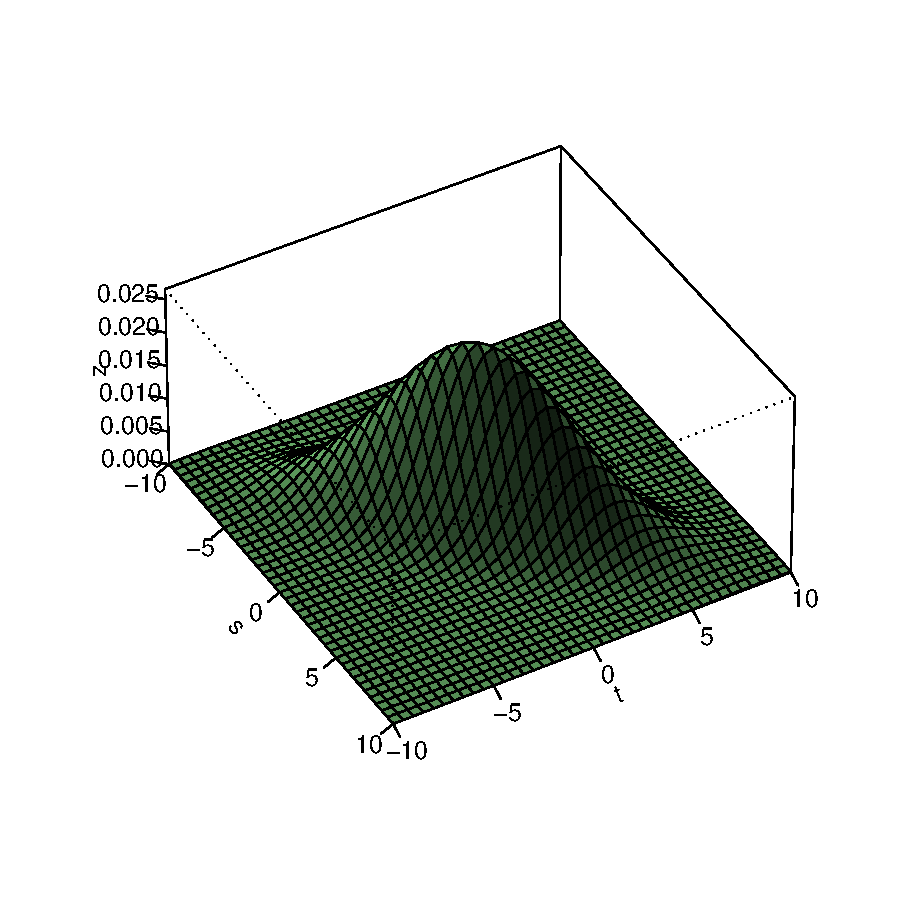
\includegraphics[width=4in]{Rho8.pdf}
}
\caption{Bivariate Normal Density, $\rho=0.8$}
\label{rho8}
\end{figure}

Again we see a bell shape, but in this case ``narrower.''  In fact, you
can see that when $X_1$ (s) is large, $X_2$ (t) tends to be large too,
and the same for ``large'' replaced by small.  By contrast, the surface
near (5,5) is much higher than near (5,-5), showing that the random
vector $(X_1, X_2)$ is near (5,5) much more often than (5,-5).

All of this reflects the high correlation (0.8) between the two variables.
If we were to continue to increase $\rho$ toward 1.0, we would see the
bell become narrower and narrower, with $X_1$ and $X_2$ coming closer
and closer to a linear relationship, one which can be shown to be

\begin{equation}
X_1 - \mu_1 = \frac{\sigma_1}{\sigma_2} (X_2 - \mu_2)
\end{equation}

In this case, that would be

\begin{equation}
X_1 = \sqrt{\frac{10}{15}} X_2 = 0.82 X_2
\end{equation}

\subsubsection{Properties of Multivariate Normal Distributions}
\label{mvnormproperties}

\begin{theorem}
\label{mvnormtheorem}

Suppose $X = (X_1,...,X_k)$ has a multivariate normal distribution with
mean vector $\mu$ and covariance matrix $\Sigma$.  Then:

\begin{itemize}

\item [(a)] The contours of $f_X$ are k-dimensional ellipsoids.  In the
case k = 2 for instance, where we can visualize the density of X as a
three-dimensional surface, the contours for points at which the bell has
the same height (think of a topographical map) are elliptical in shape.
The larger the correlation (in absolute value) between $X_1$ and $X_2$,
the more elongated the ellipse.  When the absolute correlation reaches
1, the ellipse degenerates into a straight line.

\item [(b)] Let A be a constant (i.e. nonrandom) matrix with k columns.
Then the random vector Y = AX also has a multivariate normal
distribution.\footnote{Note that this is a generalization of the
material on affine transformations on page \pageref{affine}.} 

The parameters of this new normal distribution must be $EY = A \mu$ 
and $Cov(Y) = A \Sigma A'$,  by (\ref{eaw}) and (\ref{covawaprime}).
   
\item [(c)] If $U_1,...,U_m$ are each univariate normal and they are
independent, then they jointly have a multivariate normal distribution.
(In general, though, having a normal distribution for each $U_i$ does
not imply that they are jointly multivariate normal.)  

\item [(d)] Suppose W has a multivariate normal distribution.  The
conditional distribution of some components of W, given other
components, is again multivariate normal.

\end{itemize}

\end{theorem}

Part [(b)] has some important implications:

\begin{itemize}

   \item [(i)] The lower-dimensional marginal distributions are also
   multivariate normal.  For example, if k = 3, the pair $(X_1,X_3)'$
   has a bivariate normal distribution, as can be seen by setting 

   \begin{equation} A = \left ( \begin{array}{ccc} 1 & 0 & 0\\ 0 & 0 & 1
   \end{array} \right )     \end{equation}

   in (b) above.
   
   \item [(ii)] Scalar linear combinations of X are normal.  In other
   words, for constant scalars $a_1,...,a_k$, set $a = (a_1,...,a_k)'$.
   Then the quantity $Y = a_1 X_1 +...+ a_k X_k$ has a univariate normal
   distribution with mean  $a' \mu$ and variance $a' \Sigma a$. 

   \item [(iii)] Vector linear combinations are multivariate normal.
   Again using the case k = 3 as our example, consider $(U,V)' =
   (X_1-X_3,X_2-X_3)$.  Then set

   \begin{equation}
   A = 
      \left (
      \begin{array}{ccc}
      1 & 0 & -1\\
      0 & 1 & -1   
      \end{array}
      \right )     
   \end{equation}

   \item [(iv)] The r-component random vector X has a multivariate normal
   distribution if and only if $c'X$ has a univariate normal
   distribution for all constant r-component vectors c.

\end{itemize}

In R the density, cdf and quantiles of the multivariate normal
distribution are given by the functions {\bf dmvnorm()}, {\bf pmvnorm()} 
and {\bf qmvnorm()} in the library {\bf mvtnorm}.  You can simulate a
multivariate normal distribution by using {\bf mvrnorm()} in the library
{\bf MASS}.

\subsubsection{The Multivariate Central Limit Theorem}

The multidimensional version of the Central Limit Theorem holds.  A sum
of independent identically distributed ({\it iid}) random vectors has an
approximate multivariate normal distribution.  Here is the theorem:

\begin{theorem}

Suppose $X_1, X_2, ...$ are independent random {\it vectors}, all having
the same distribution which has mean vector $\mu$ and covariance matrix
$\Sigma$.  Form the new random vector $T = X_1+...+X_n$.  Then for large
n, the distribution of T is approximately normal with mean $n \mu$ and
covariance matrix $n \Sigma$.

\end{theorem}


For example, since a person's body consists of many different
components, the CLT (a non-independent, non-identically version of it)
explains intuitively why heights and weights are approximately bivariate
normal.  Histograms of heights will look approximately bell-shaped, and
the same is true for weights.  The multivariate CLT says that
three-dimensional histograms---plotting frequency along the ``Z'' axis
against height and weight along the ``X'' and ``Y'' axes---will be
approximately three-dimensional bell-shaped.

The proof of the multivariate CLT is easy, from Property (iv) above.
Say we have a sum of iid random vectors:

\begin{equation}
S = X_1 + ... + X_n
\end{equation}

Then 

\begin{equation}
c'S = c'X_1 + ... + c'X_n
\end{equation}

Now on the right side we have a sum of iid {\it scalars}, not vectors,
so the univariate CLT applies!  We thus know the right-hand side is a
approximately normal for all c, which means $c'S$ is also approximately
normal for all c, which then by (iv) above means that S itself is
approximately multivariate normal.

\subsubsection{Example:  Finishing the Loose Ends from the Dice Game}

Recall the game example in Section \ref{dicegame}:

Suppose we roll a die 50 times.  Let X denote the number of rolls in
which we get one dot, and let Y be the number of times we get either two
or three dots.  For convenience, let's also define Z to be the number of
times we get four or more dots, though our focus will be on X and Y.
Suppose also that we win \$5 for each roll of a one, and \$2 for each
roll of a two or three.

Our analysis relied on the vector (X,Y,Z)' having an approximate
multivariate normal distribution.  Where does that come from?  Well,
first note that the exact distribution of (X,Y,Z)' is multinomial.  Then
recall (\ref{multinomsumindic}).  The latter makes (X,Y,Z)' a sum of
iid vectors, so that the multivariate CLT applies.

